\section{Ejercicio 4}
\subsection{Arquitectura}
\begin{center}
    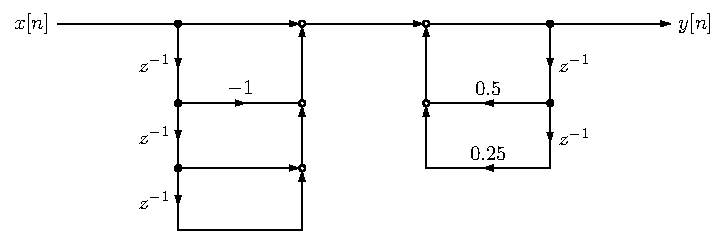
\includegraphics[width=\linewidth]{../iir_filter/draw/draw.pdf}
\end{center}

\subsection{Cálculo de la cantidad de bits de salida}
Se consideró que las 4 muestras en X podían tener los valores límites, es decir, -128 y 127. De donde se obtiene un mínimo de $4\cdot(-128) = -512$ y un máximo de $4\cdot127 = 508$.\\

Para el caso de las muestras en Y se tuvieron en cuenta los extremos considerados previamente, de donde se obtuvo: $0.75\cdot(-512) = -384$ y $0.75\cdot508 = 381$.\\

A partir de estos extremos, se calculó el rango:
\[
    rango =
    \begin{cases}
        Min = -512-384 = -896\\
        Max = 508+381 = 889\\
        Total = 889 - (-896) + 1 = 1786
    \end{cases}
\]
Para representar dicho rango se requieren 11 bits.

\subsection{Código}
\inputminted[fontsize=\footnotesize]{systemverilog}{../iir_filter/rtl/iir_filter.sv}

\subsection{Verificación}
Se plantearon 6 TCs, los cuales son:
\begin{itemize}
    \item TC001: Entrada constante
        \begin{minted}[fontsize=\footnotesize]{python}
async def TC001(dut):
    await init_rtl(dut)
    dut.i_data.value = -128

    for _ in range(200):
        await RisingEdge(dut.i_clock)
        \end{minted}

    \item TC002: Cambio aleatorio en la entrada cada cinco clocks
        \begin{minted}[fontsize=\footnotesize]{python}
async def TC002(dut):
    await init_rtl(dut)

    for _ in range(rnd.randint(5,20)):
        await RisingEdge(dut.i_clock)

    for _ in range(500):
        dut.i_data.value = rnd.randint(-100,100)
        for _ in range(5):
            await RisingEdge(dut.i_clock)
        \end{minted}

    \item TC003: Onda senoidal de 50kHz
        \begin{minted}[fontsize=\footnotesize]{python}
async def TC003(dut):
    await init_rtl(dut)
    await run_sinusoidal_wave(dut = dut, waiting_clocks = 10000, freq_in_hz = 50000, amplitude = 20)
        \end{minted}

    \item TC004: Onda senoidal de 1MHz
        \begin{minted}[fontsize=\footnotesize]{python}
async def TC004(dut):
    await init_rtl(dut)
    await run_sinusoidal_wave(dut = dut, waiting_clocks = 1000, freq_in_hz = 1000000, amplitude = 20)
        \end{minted}

    \item TC005: Onda senoidal de 10MHz
        \begin{minted}[fontsize=\footnotesize]{python}
async def TC005(dut):
    await init_rtl(dut)
    await run_sinusoidal_wave(dut = dut, waiting_clocks = 1000, freq_in_hz = 10000000, amplitude = 20)
        \end{minted}

    \item TC006: Reset y recuperación con una onda cuadrada
        \begin{minted}[fontsize=\footnotesize]{python}
async def TC006(dut):
    await init_rtl(dut)

    timespace     = np.linspace(0, 10000*10e-9, 10000, endpoint=False)
    square_signal = signal.square(2*np.pi*1e6*timespace, duty = 0.5)
    reset_times   = 3

    for value in square_signal:
        await RisingEdge(dut.i_clock)
        dut.i_data.value = 20*int(value)
        if (rnd.randint(0,1200) == 0) and (reset_times > 0):
            await reset_rtl(dut)
            reset_times -= 1
        \end{minted}
\end{itemize}

Las funciones common para los tests fueron:
\begin{minted}[fontsize=\footnotesize]{python}
async def init_rtl(dut):
    cocotb.start_soon(Clock(dut.i_clock, 10, units="ns").start())
    tester = RtlModel(dut)

    dut.i_reset.value = 0
    dut.i_data.value  = 0
    await RisingEdge(dut.i_clock)
    await RisingEdge(dut.i_clock)
    dut.i_reset.value = 1
    tester.start()
    await RisingEdge(dut.i_clock)
    await RisingEdge(dut.i_clock)
    dut.i_reset.value = 0
    await RisingEdge(dut.i_clock)

async def reset_rtl(dut):
    await RisingEdge(dut.i_clock)
    dut.i_reset.value = 0
    await RisingEdge(dut.i_clock)
    dut.i_reset.value = 1
    await RisingEdge(dut.i_clock)
    dut.i_reset.value = 0

async def run_sinusoidal_wave(dut: SimHandleBase, waiting_clocks: int, freq_in_hz: int, amplitude: int):
    sampling_freq = 1/(10e-9)
    for i in range(waiting_clocks):
        await RisingEdge(dut.i_clock)
        dut.i_data.value = int(amplitude*np.sin(2*np.pi*i*(freq_in_hz/sampling_freq)))

\end{minted}

La principal función de verificación, la cual se encuentra dentro del objeto RtlModel, fue:
\begin{minted}[fontsize=\footnotesize]{python}
    async def _check(self) -> None:
        while True:
            await RisingEdge(self.dut.i_clock)
            if (int(self.dut.i_reset.value) == 1):
                self.clear_monitors()
                continue

            result  = self.input_monitor.get_n_sample(0) .to_signed()
            result -= self.input_monitor.get_n_sample(1) .to_signed()
            result += self.input_monitor.get_n_sample(2) .to_signed()
            result += self.input_monitor.get_n_sample(3) .to_signed()
            result += self.output_monitor.get_n_sample(2).to_signed()//4
            result += self.output_monitor.get_n_sample(1).to_signed()//2

            # print(f'Result: {result} | Got: {self.output_monitor.get_n_sample(0).to_signed()} ')
            assert result == self.output_monitor.get_n_sample(0).to_signed()

            _ = self.output_monitor.values.get_nowait()
            _ = self.input_monitor.values.get_nowait()
\end{minted}

El entorno completo se puede encontrar en este \href{https://github.com/msebgarcia/DDA2024/tree/main/GP01/iir_filter/tb}{link de github}, estando los TCs en el archivo \href{https://github.com/msebgarcia/DDA2024/blob/main/GP01/iir_filter/tb/test_module.py}{test\_module.py} y el modelo del RTL en \href{https://github.com/msebgarcia/DDA2024/blob/main/GP01/iir_filter/tb/model.py}{model.py}.


